\section{Simplified ByteNet}

The implementation of the ByteNet model spends $37\%$ of its time waiting for data transfer between GPU and CPU and even more time waiting on the TensorFlow service. This is because of the large amount of weights and operations that is used in the ByteNet model.

To solve this issue a simplified version of ByteNet has been created. This uses less weights and less operations than ByteNet, but remain true to principals behind ByteNet. Those principals is running in linear time, parallelize over both sequence and observations, have be resolution persistent meaning that the size of the encoded representation scales with the sequence length. The simplified version also maintains the bottleneck of 200 dimensions that ByteNet has in its dilated-convolution layer.

The idea behind this is simple, if the initial embedding dimensionality is set to 200 then the compression and decompression layers that exists before and after the dilated convolution are not needed. Of cause these layers adds non-linearities and weights to the model, thus one should not expect the model to perform equally well. Instead the model should before almost as well and be significantly faster.

\begin{figure}[H]
    \centering
    \begin{subfigure}[b]{0.45\textwidth}
        \centering
        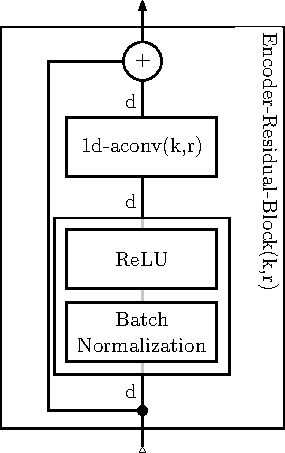
\includegraphics[scale=1]{theory/bytenet-small-residual-block.pdf}
        \caption{Residual Block used in encoder.}
    \end{subfigure}
    ~ %
    \begin{subfigure}[b]{0.45\textwidth}
        \centering
        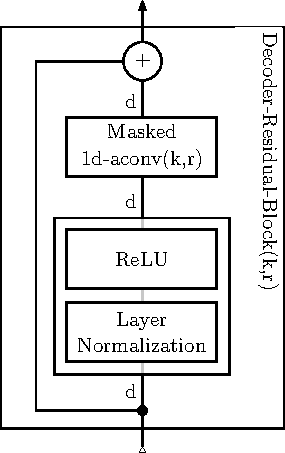
\includegraphics[scale=1]{theory/bytenet-small-residual-block-causal.pdf}
        \caption{Residual Block used in decoder.}
    \end{subfigure}
    \caption{The residual blocks used in the Simplified ByteNet model. The blocks are denoted by Encoder-Residual-Block$(k,r)$ and Decoder-Residual-Block$(k,r)$, where $k$ is the kernel width and $r$ is the dilation rate.}
    \label{fig:result:simple-bytenet:residual-block}
\end{figure}

In terms of weights the simplified ByteNet model has approximately $\sfrac{5}{9}$ times less weights than the ByteNet model. The simplified ByteNet model also has approximately one third of the operations as the ByteNet model. Based on these parameters one should expect less transfer time and less time spend waiting for the TensorFlow service.

The simplified ByteNet model was validated identically to the how the ByteNet model was validated. The results (appendix \ref{appendix:result:bytenet-small}) where very similar with some minor differences. Memorizing WMT NewsTest took fewer iterations, this is likely because there are fewer parameters. The simplified ByteNet model learned the synthetic digits problem better, with a misclassification error of $0.25$. An explanation could for the improved misclassification error is that the the simplified ByteNet model has fewer parameters and non-linear transformation, this might make it overfit less.

\subsection{Performance Profiling}

To compare the performance of the simplified ByteNet model with the normal ByteNet model, the performance experiment from the normal ByteNet model was repeated using the simplified ByteNet model. This experiment learns the WMT NewsTest dataset over 300 epochs. Both a 1 GPU and a 4 GPU setup was used in the experiments.

\begin{figure}[h]
    \centering
    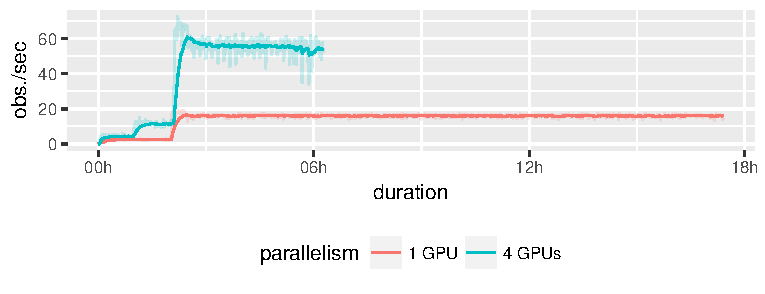
\includegraphics[scale=1]{bytenet-small/timing-gpus.pdf}
    \caption{Comparing observations per second, depending on the number of GPUs used.}
    \label{fig:result:simple-bytenet:timing-gpus}
\end{figure}

Measuring the total time spend and the observations per second as seen in figure \ref{fig:result:simple-bytenet:timing-gpus} reveals that the simplified ByteNet model is faster. On 1 GPU the simplified ByteNet model is about $20\%$ faster. This is quite far from the best case $66\%$, that one would get from reducing the number of operation to $\sfrac{1}{3}$.

On 1 GPU there is no data transfer, thus it is only the TensorFlow service and the computation that takes time. Assuming the actual computation time is not the most time consuming part, reducing the number of operations to $\sfrac{1}{3}$ should result in a $\sfrac{2}{3}$ computational performance gain. This is of cause an approximation as there is still the embedding layer, the concatenation of encoding and decoding, and the final output layer, thus $\sfrac{2}{3}$ the operations is an upper bound.

Comparing the time spend in the 1 GPU experiment and the 4 GPU experiment, and because very little data transfer happens when using 1 GPU. The data shows that approximately $40\%$ time is spend transferring data. This is approximately the same as the $37\%$ in the normal ByteNet model. The number of weights is reduced by $\sfrac{5}{9}$, thus one would expect the transfer time to be reduced by this order, however that is not the case.

\begin{figure}[h]
    \centering
    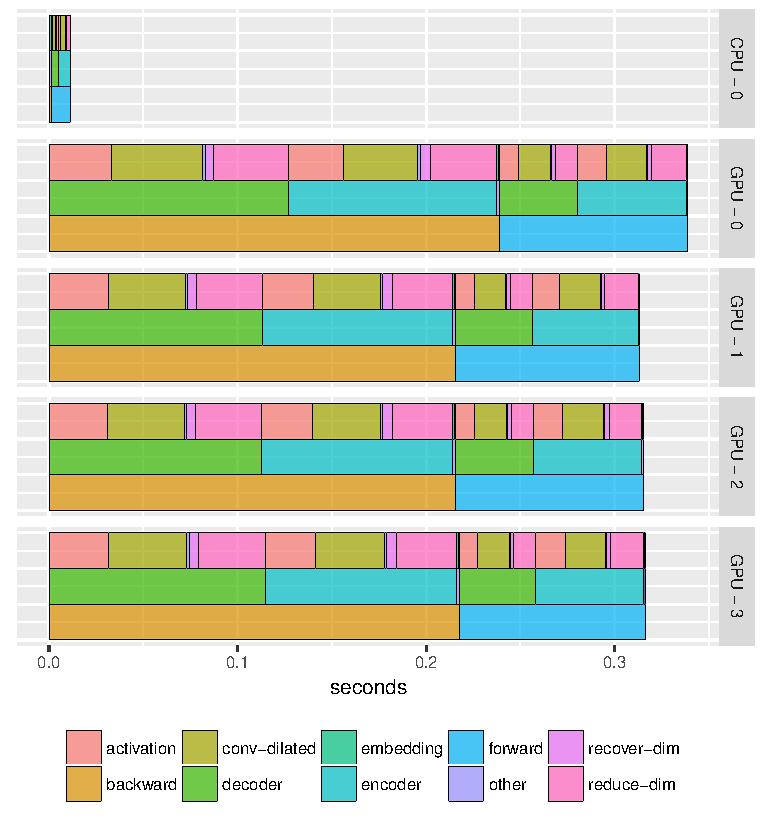
\includegraphics[scale=1]{bytenet-small/profile-grouped-gpu4.pdf}
    \caption{Shows time spend executing operations in each part of the ByteNet model, this excludes the waiting time. Each part exists in a hierarchy, which is visualized as levels. The bottom level is the least detailed level, it just splits the model in the backward and forward pass. The next level, splits the model in the encoder and decoder. The last level at the top, primarily splits the Simplified ByteNet Residual Blocks.}
    \label{fig:result:simple-bytenet:profile-grouped}
\end{figure}

Finally the TensorFlow profiler can be used to investigate what takes time. When processed the results are similar to those from the normal ByteNet model, see figure \ref{fig:result:simple-bytenet:profile-grouped}.

From figure \ref{fig:result:simple-bytenet:profile-grouped} that much of the time is spend in the \textit{activation layer}. The \textit{activation layer} is the layer that contains the normalization and ReLU operation. This validates the idea that it is the number of operations and not the operations themselves that cost in terms of time. The dilated convolution (called \textit{conv-dilated}) is a much more complex operation than normalization or ReLU, but TensorFlow implements it using just a few operations, thus it doesn't consume that much time. As mentioned earlier the TensorFlow team is aware of this performance issue, and tries to solve it my automatically compiling GPGPU (CUDA or OpenCL) kernels that combines multiple operations into one, but this is still very experimental and doesn't yet provide a performance when using multiple GPUs \cite{citation-needed}.

\clearpage
\subsection{WMT Translation Task}

The Europarl v7 dataset is used to train the simplified ByteNet model. The setup is identical to that previously used to train the normal ByteNet model. The internal dimensionality is 400, the Adam optimizer is used with a learning rate of 0.0003, and the mini-batch size is $4 \cdot 16 = 64$ observations, 4 GPUs with synchronized updates was used, and the model ran 13 epochs over the Europarl v7 dataset.

\begin{figure}[h]
    \centering
    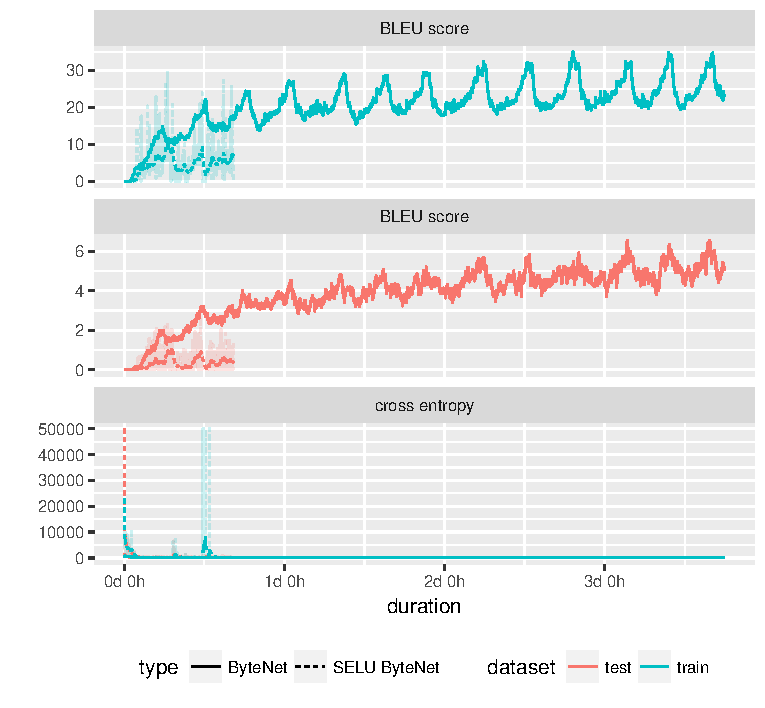
\includegraphics[scale=1]{bytenet-small/europarl.pdf}
    \caption{Shows BLEU score and cross entropy loss for the Simplified ByteNet model, trained on Europarl v7 and tested on WMT NewsTest 2015. Both training and test measures are calculated on a randomly sampled mini-batch from each dataset. The exponential smoothing used a forget factor of $0.05$. The raw data for the non-simplified ByteNet model is now shown.}
    \label{fig:result:bytenet-small:europarl}
\end{figure}

The simplified ByteNet model uses almost 24 hours less training time. However, it also learns at a slower rate, thus in terms of BLUE score given the time spend learning the normal ByteNet model is actually much faster.

An interesting observation is that the simplified ByteNet model also overfits a lot more than the normal ByteNet model. This contradicts most intuition about overfitting, which usually is the more weights, layers, and non-linearities, the easier it is to make the model overfit. The simplified ByteNet model has less of all three factors, thus there is no reason to expect the simplified ByteNet model to overfit more.

It is not clear why this overfitting happens, but it is very likely a contributing factor to why the test BLEU score isn't isn't better. However, this can not be the entire explanation, as also the training BLEU score is worse. If anything, overfitting should cause a higher training BLEU score as regularization typically increases the training loss in order to decrease the test loss.

Possible regularization methods are L1, L2, and dropout. Particularly, L1 regularization could be interesting in the first 5 \textit{residual blocks}, as these layers likely performs some characters-to-word encoding. Such an encoding should be very sparse, L1 regularization would enforce such a sparsity.

The translations as shown in table \ref{table:result:bytenet-small:translations} are rather bad, they have little connection to the source sequence and there a tendency for the sequence ``Mr \textit{insert name}'' to appear without context. The poor translations can likely be attributed to the server overfitting. \todo{total BLEU score is $0.55$}

\begin{table}[h]
\centering
\begin{tabular}{l|r|p{10cm}}
0 & source & Die formelle Anerkennung der Arbeitsrechte als Menschenrechte - und die Erweiterung des Schutzes der Bürgerrechte als Schutz gegen Diskriminierung bei der Schaffung von Arbeitnehmervertretungen - ist längst überfällig. \\[0.1cm]
& target & The formal recognition of labor rights as human rights - and the extension of civil rights protections to prevent discrimination against labor organizing - is long overdue. \\[0.1cm]
& translation & However, the recommendation of jobs and generations and proposes the promotion of gross regions of the world growth to prodictively rejecting the rejection of the representative of the representative increase' . \\[0.1cm]
& BLEU & 0.00 \\[0.1cm] \hline

1 & source & Die Premierminister Indiens und Japans trafen sich in Tokio. \\[0.1cm]
& target & India and Japan prime ministers meet in Tokyo \\[0.1cm]
& translation & Mr Pieper and the independence of Singapore in London. \\[0.1cm]
& BLEU & 0.00 \\[0.1cm] \hline

2 & source & Er wird beschuldigt, am 7. Juni 2013 eine Frau im Scotland's Hotel in Pitlochry in Perthshire vergewaltigt zu haben. \\[0.1cm]
& target & He is alleged to have raped a woman at the Scotland's Hotel in Pitlochry in Perthshire on June 7, 2013. \\[0.1cm]
& translation & Madam President, I should like to contribute to Mr President Mr President in his report. \\[0.1cm]
& BLEU & 0.00 \\[0.1cm]
\end{tabular}
\caption{Cherry-picked translations from WMT NewsTest.}
\label{table:result:bytenet-small:translations}
\end{table}

